\documentclass[10pt,oneside,english,a4paper]{article}

\usepackage[english]{babel}
\usepackage{fontenc} 
\usepackage{inputenc}
\usepackage{graphicx}
\usepackage{url} 
\usepackage{hyperref} 
\usepackage{cite}
\usepackage{titlesec}
\usepackage{listings}
\usepackage{titling}
\usepackage[table,xcdraw]{xcolor}
\usepackage{multicol}
\usepackage{tabto}
\usepackage{comment}

% \tab - huge space
% \quad - small space, stackable

\pagestyle{headings}
\title{\huge \textbf{Slovak University of Technology in Bratislava
\\Faculty of Informatics and Information Technologies in Bratislava}\\
\ \\
Principles of information security\\
\ \\
Freely distributed password cracking tools}


\author{Ákos Lévárdy}

\begin{document}

\maketitle

\pagebreak

\tableofcontents

\pagebreak

\section{Topic of the project: \\Freely distributed password cracking tools}
In my topic I will be focused on freely distributed password cracking tools. Firstly, I will describe how passwords are encrypted or hashed. Passwords are used everywhere for user authentication, which is a widely adopted method due to its intuitive logic and ease of implementation for developers. 

Despite their popularity, passwords pose security risks as password crackers are crafted to extract credentials from compromised data obtained through breaches or hacks.

\section{What is password cracking?}

Most password-based authentication systems do not store a user’s actual password. Instead, they store a password hash, which is the result of sending the password and a random value called a salt through a hash function.

I will compare different hash functions and describe how they work when in use. Basically, hash functions are designed to be one way. This means that it is very difficult to get the original password from the hashed output. 

It is important to know that hash functions are producing the same output for the same input. Comparing two hashes of a password is eventually the same as comparing two real passwords.


\subsection{Password cracking tools}

There are many different tools for password cracking.\\
The most popular ones are: 
\begin{multicols}{2}
\begin{itemize}
    \item Hashcat
    \item John the Ripper
    \item Brutus
    \item Wfuzz
    \item THC Hydra
\end{itemize}
\columnbreak
\begin{itemize}
    \item Meduza
    \item RainbowCrack
    \item OphCrack
    \item L0phtCrack
    \item Aircrack-ng
\end{itemize}
\end{multicols}

I will be comparing two of these password cracking tools – Hashcat and John the Ripper, analyze them, see how they work and then compare their performance. 


\section{Types of attacks on passwords}
There are various types of attacks on passwords, and they can be categorized into different methods based on their techniques. 
\\
Most common types of password attacks:
\begin{itemize}
\item Brute Force Attack - This involves trying all possible combinations of passwords until the correct one is found.
\item Dictionary Attack - Attackers use a predefined list of common words, dictionaries to try and guess the password.
\item Rainbow Table Attack - A precomputed table containing the hash values of commonly used passwords. This attack compares these hashes with the target system's stored password hashes to find a match.
\item Phishing – This attack tries to trick individuals into revealing their passwords by posing as a trustworthy entity.
\item Keylogging - Malicious software or hardware records keystrokes without the user noticing it and capturing sensitive information such as usernames and passwords.
\item Man-in-the-Middle (MitM) Attack - Intercepting communication between two sides to capture information, including passwords and usernames.
\item Shoulder Surfing - Observing someone entering their password without their knowledge.
\end{itemize}


\section{Progress report 1}
For the first progress report I will analyse the different hashing algorithms and compare the types of attacks on passwords. I will write about the history of some tools for password cracking and about how to defend our passwords with password managers and other tools. 

\section{Progress report 2}
For the second progress report I will test two password cracking tools and then compare how they work and their performance. I will use John the Ripper and Hashcat on Kali Linux after I set up a Virtual box for it.

\clearpage


\section{Authentication}
For authenticating a user there are 2 different types. One-factor authentication relies solely on one type of information for verification (usually a password), two-factor authentication enhances security by requiring two different types of information, making it harder for unauthorized users to gain access even if they have obtained one factor (password).

\begin{itemize}
\item One-Factor Authentication (1FA):\\
\begin{itemize}
\item In one-factor authentication, only one type of information is required to verify the identity of the user.
\item Typically, this involves something the user knows, such as a password or a PIN.
\item It's the simplest form of authentication and is commonly used in many basic systems.
\end{itemize}

\item Two-Factor Authentication (2FA):\\
\begin{itemize}
\item Two-factor authentication requires two different types of information to authenticate the user.
\item These factors usually fall into one of three categories: something the user knows (password), something the user has (smartphone or a security token), or something the user is (biometric data like fingerprints or facial recognition).
\item By requiring two factors, 2FA adds an extra layer of security beyond just a password, making it more difficult for unauthorized users to gain access.
\item Common implementations of 2FA include receiving a text message with a code, using an authenticator app, or using biometric authentication along with a password.
\end{itemize}
\end{itemize}


\section{Password-Hashing Schemes - PHS}
Everyday tasks involve the use of computers, and many people use the services that are offered. The most popular method for authenticating users on the web is one-factor authentication, which consists of a password and a username.
\\\\
Unfortunately, attackers take advantage of weak password management procedures to reveal users' credentials, which hurts both users and providers.
In the majority of these cases, the user data was either processed directly by a cryptographic hash function or kept in cleartext.

\subsection{Password-Hashing procedures}
We use password-hashing procedures to secure this user-related data.
Currently, the Password-Based Key Derivation Function 2 (PBKDF2) standard primitive is in use, however other popular schemes like Blowfish cipher - Bcrypt and Scrypt are also in use.
The development of parallel computing has made it possible for multiple password-hash cracking attempts.
\\\\
For the purpose of developing new, widely-acceptable password-hashing algorithms that are more safe and efficient, the global cryptography community organized the Password Hashing Competition (PHC). PHC improved our understanding of hashing passwords. Security flaws were discovered through more investigation, and new methods were subsequently developed.

\subsection{Background Theory}
A password is a secret that is straightforward for the user to remember and consists of just a few printed characters. In computer systems, passwords are frequently used for user authentication. For each account, the system keeps track of the user's identity and password. The individual then uses this information to log in and access the service.
\\\\
The creation of cryptographic keys is another use for passwords. Based on an input password, the Key-Derivation Functions (KDF) generates a variety of cryptographic keys. KDFs primarily serve for session data encryption, and cryptographic keys are applied by encryption/decryption functions.
\\\\
Cryptographic keys play a critical role in ensuring the security of data and communications in cryptographic systems. They enable encryption, decryption, digital signing, and authentication, helping to protect sensitive information from unauthorized access, tampering, or interception. \\
Proper key management practices are essential to maintaining the effectiveness and security of cryptographic systems.
\\\\
Encryption converts plaintext into ciphertext using an encryption algorithm and a key, while decryption reverses this process to recover the original plaintext. 
These processes play a crucial role in protecting data confidentiality and integrity, ensuring that only authorized users can access and understand the encrypted information.


\subsection{Key-Derivation Function}
A key derivation function (KDF) is a cryptographic tool used to derive one or more secret keys from a single, fixed-length secret value, such as a master key or a passphrase.
\begin{itemize}
\item The KDF takes as input the secret value and possibly some additional parameters, such as a salt (random value) or context information.
\item The KDF expands the input secret into one or more longer keys. This expansion process typically involves applying a cryptographic hash function or a more complex cryptographic algorithm repeatedly to the input, potentially mixing in the salt or other parameters. The goal is to generate keys that are unpredictable and have high entropy (randomness).
\item The output of the KDF is one or more derived keys, which can be used for various cryptographic purposes, such as encryption, authentication, or generating other cryptographic parameters.

\item Security Properties: \\
A strong KDF should include the following security features:
	\begin{itemize}        
		\item Key Derivation: Both the derived keys and the input secret must be computationally independent of one another.
	        \item Resistance to Attacks: The KDF should resist various cryptographic attacks, such as brute-force attacks (trying all possible inputs) and pre-image attacks (deriving the input from the output).
	        \item Salt and Context Sensitivity: Incorporating a salt and context information can enhance the security of the derived keys by making them unique to each application or usage scenario.
	\end{itemize}

\item Essentially, a key derivation function offers a safe method for producing cryptographic keys from a single secret value, guaranteeing the confidentiality and integrity of the derived keys and making them appropriate for usage in cryptographic protocols and applications.
\end{itemize}

\subsection{Password Security Risks and Vulnerabilities}
When people create passwords for their accounts, they often use simple ones that are just eight characters long. These passwords are not very secure because they're easy to guess. 
\\\\
Hackers can use a method called exhaustive search to try every possible combination of characters until they find the right password. Once they do, they can access the account just like the real user. Even graphical passwords, where you draw patterns or pick images, can be easy for hackers to figure out because they don't provide much security.

\subsection{Password-Based Key Derivation Function 2 - PBKDF2}
PBKDF2 is a widely used key derivation function that's designed to derive cryptographic keys from a password or passphrase.
Hashing-based techniques are the standard option for establishing password protection. The primary methods for making KDFs possible are keyed-hash message authentication codes (HMACs) and cryptographic hash functions that translate a password into one or more secret keys.
\\\\
PBKDF2 uses pseudo-random functions (PRF), commonly implemented by HMACs.
HMAC is a specific type of PRF that's widely used in cryptographic applications for generating message authentication codes.
The SHA-256 function is the standard internal hash option for the HMAC. 
\\\\
A pseudo-random function (PRF) is a mathematical function that produces seemingly random outputs from given inputs.
Unlike truly random functions, PRFs are deterministic, meaning that the same input always produces the same output.
PRFs are designed to mimic the properties of random functions while being efficiently computable.
\\\\
The scheme parses the password and the salt as inputs.
Attacks utilizing precomputed data, such as dictionary attacks (which test hundreds of plausible combinations to determine the passphrase) and rainbow-table attacks (which make use of tables with precomputed hashes), are made more resilient by the salt. 
It typically has 8 bytes in size.\\\\
PBKDF2 steps:

\begin{itemize}
\item The salt and the password are initially processed by the HMAC. 
\item The derived key is then generated by processing the data multiple times.
\item Although 1000 iterations is the minimum required amount, given that the guideline was set in 2000, it is no longer deemed sufficient. 
\item The password and the previous HMAC result are parsed by the HMAC at each repetition.  
\item The HMAC outcomes are then XORed.
\item The outcome of the XOR operation in the last round is the final hash.
\end{itemize}

\begin{figure}[h!]
	\centering
	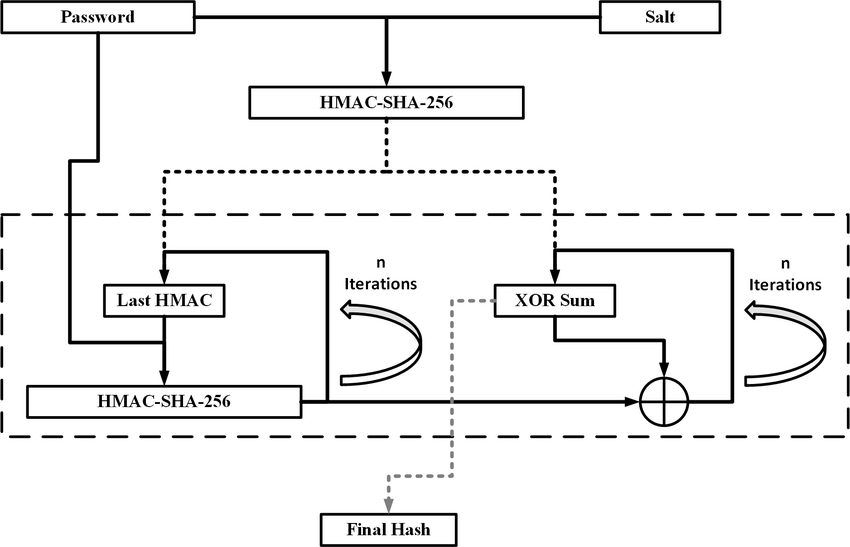
\includegraphics[scale = 0.40]{PBKDF2.png}
	\caption{PBKDF2}
	\label{}
\end{figure}

The effective hardware-based cracking has a downside because it can be created as a small hardware implementation with little RAM requirements. Therefore, on GPUs, FPGAs, and ASICs, low-cost brute-force attacks are possible. \\
In roughly one week, the most rapid attacks can crack about 65\% of common passphrases. Approximately 245,000 passwords are obtained per second by attacks on multi-FPGA devices.

\subsection{Bcrypt}
Bcrypt is the chosen password hashing system for the BSD operating system. It makes use of the Blowfish block cipher. By default, it processes passwords that are 56 bytes long and produces hashes that are 24 bytes long. The number of iterations increases exponentially as the computational power of potential attackers grows, ensuring adequate protection against brute-force attacks. Additionally, a 16-byte salt value is employed to strengthen defenses against attacks relying on rainbow tables. 
\\\\
Bcrypt steps:

\begin{itemize}
\item Initialization: Bcrypt starts by setting up the Blowfish cipher with a cost parameter, a salt (a random value), and your password. This sets up a complex system of encryption.

\item Key Schedule: Bcrypt then creates a set of subkeys based on your password. These subkeys are mixed with the original password in a special way.

\item Encryption: The salt is encrypted using the key schedule. This process repeats several times, making it harder for attackers to reverse-engineer the password.

\item Magic Value Encryption: A special value is encrypted multiple times using Blowfish. This further scrambles the data.

\item Final Hash: The final hash is created by combining the salt, cost, and the result of the encryption process
\end{itemize}

\begin{figure}[h]
	\centering
	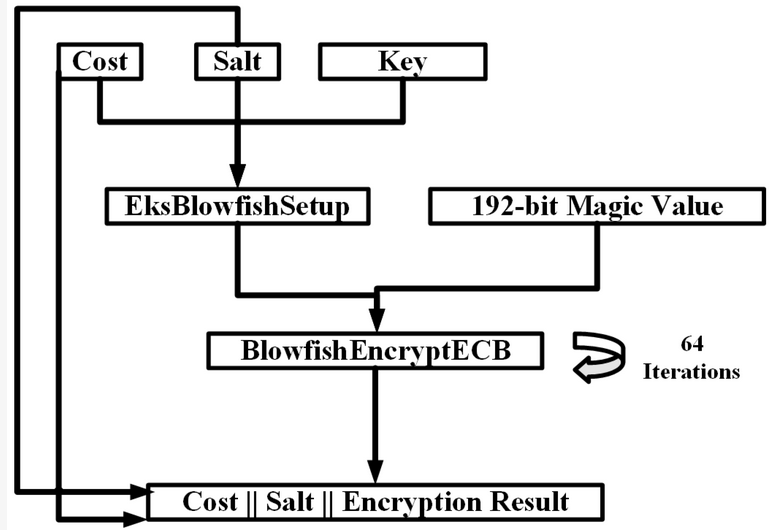
\includegraphics[scale = 0.40]{Bcrypt.png}
	\caption{Bcrypt}
	\label{}
\end{figure}

The method uses 4KB of RAM and outperforms PBKDF2 in terms of blocking parallel cracking. While the best attack discovers 20,583 passwords per second, the least expensive attack only manages 1207 cracks per second at a cost of \$99.

\subsection{Scrypt}
Scrypt is designed to be a memory-hard password hashing scheme, which means it makes it difficult for attackers to use large amounts of memory when trying to crack passwords.
\\\\
Scrypt steps: 

\begin{itemize}
\item It is based on the PBKDF2 algorithm and the Salsa stream cipher.
\item It has features like 
MFcrypt (Memory-Hard Function), 
ROMix (Rounds Mixer), 
BlockMix, and 
SMix (Sequential Memory-Hard Function).

\item To make sure all of the random values are kept in memory, ROMix creates a  bunch of them and shuffles them around.
\item BlockMix facilitates this procedure by utilizing another version of the Salsa cipher.
\item SMix uses one or more ROMix functions to further complicate matters.
\item The number of ROMix functions (parallelization parameters) determines how much time and space the process takes.
\item MFcrypt is the final step, where the key-derivation function combines the mixing function with PBKDF2 using the SHA-256 hash function.
\end{itemize}

\begin{figure}[h]
	\centering
	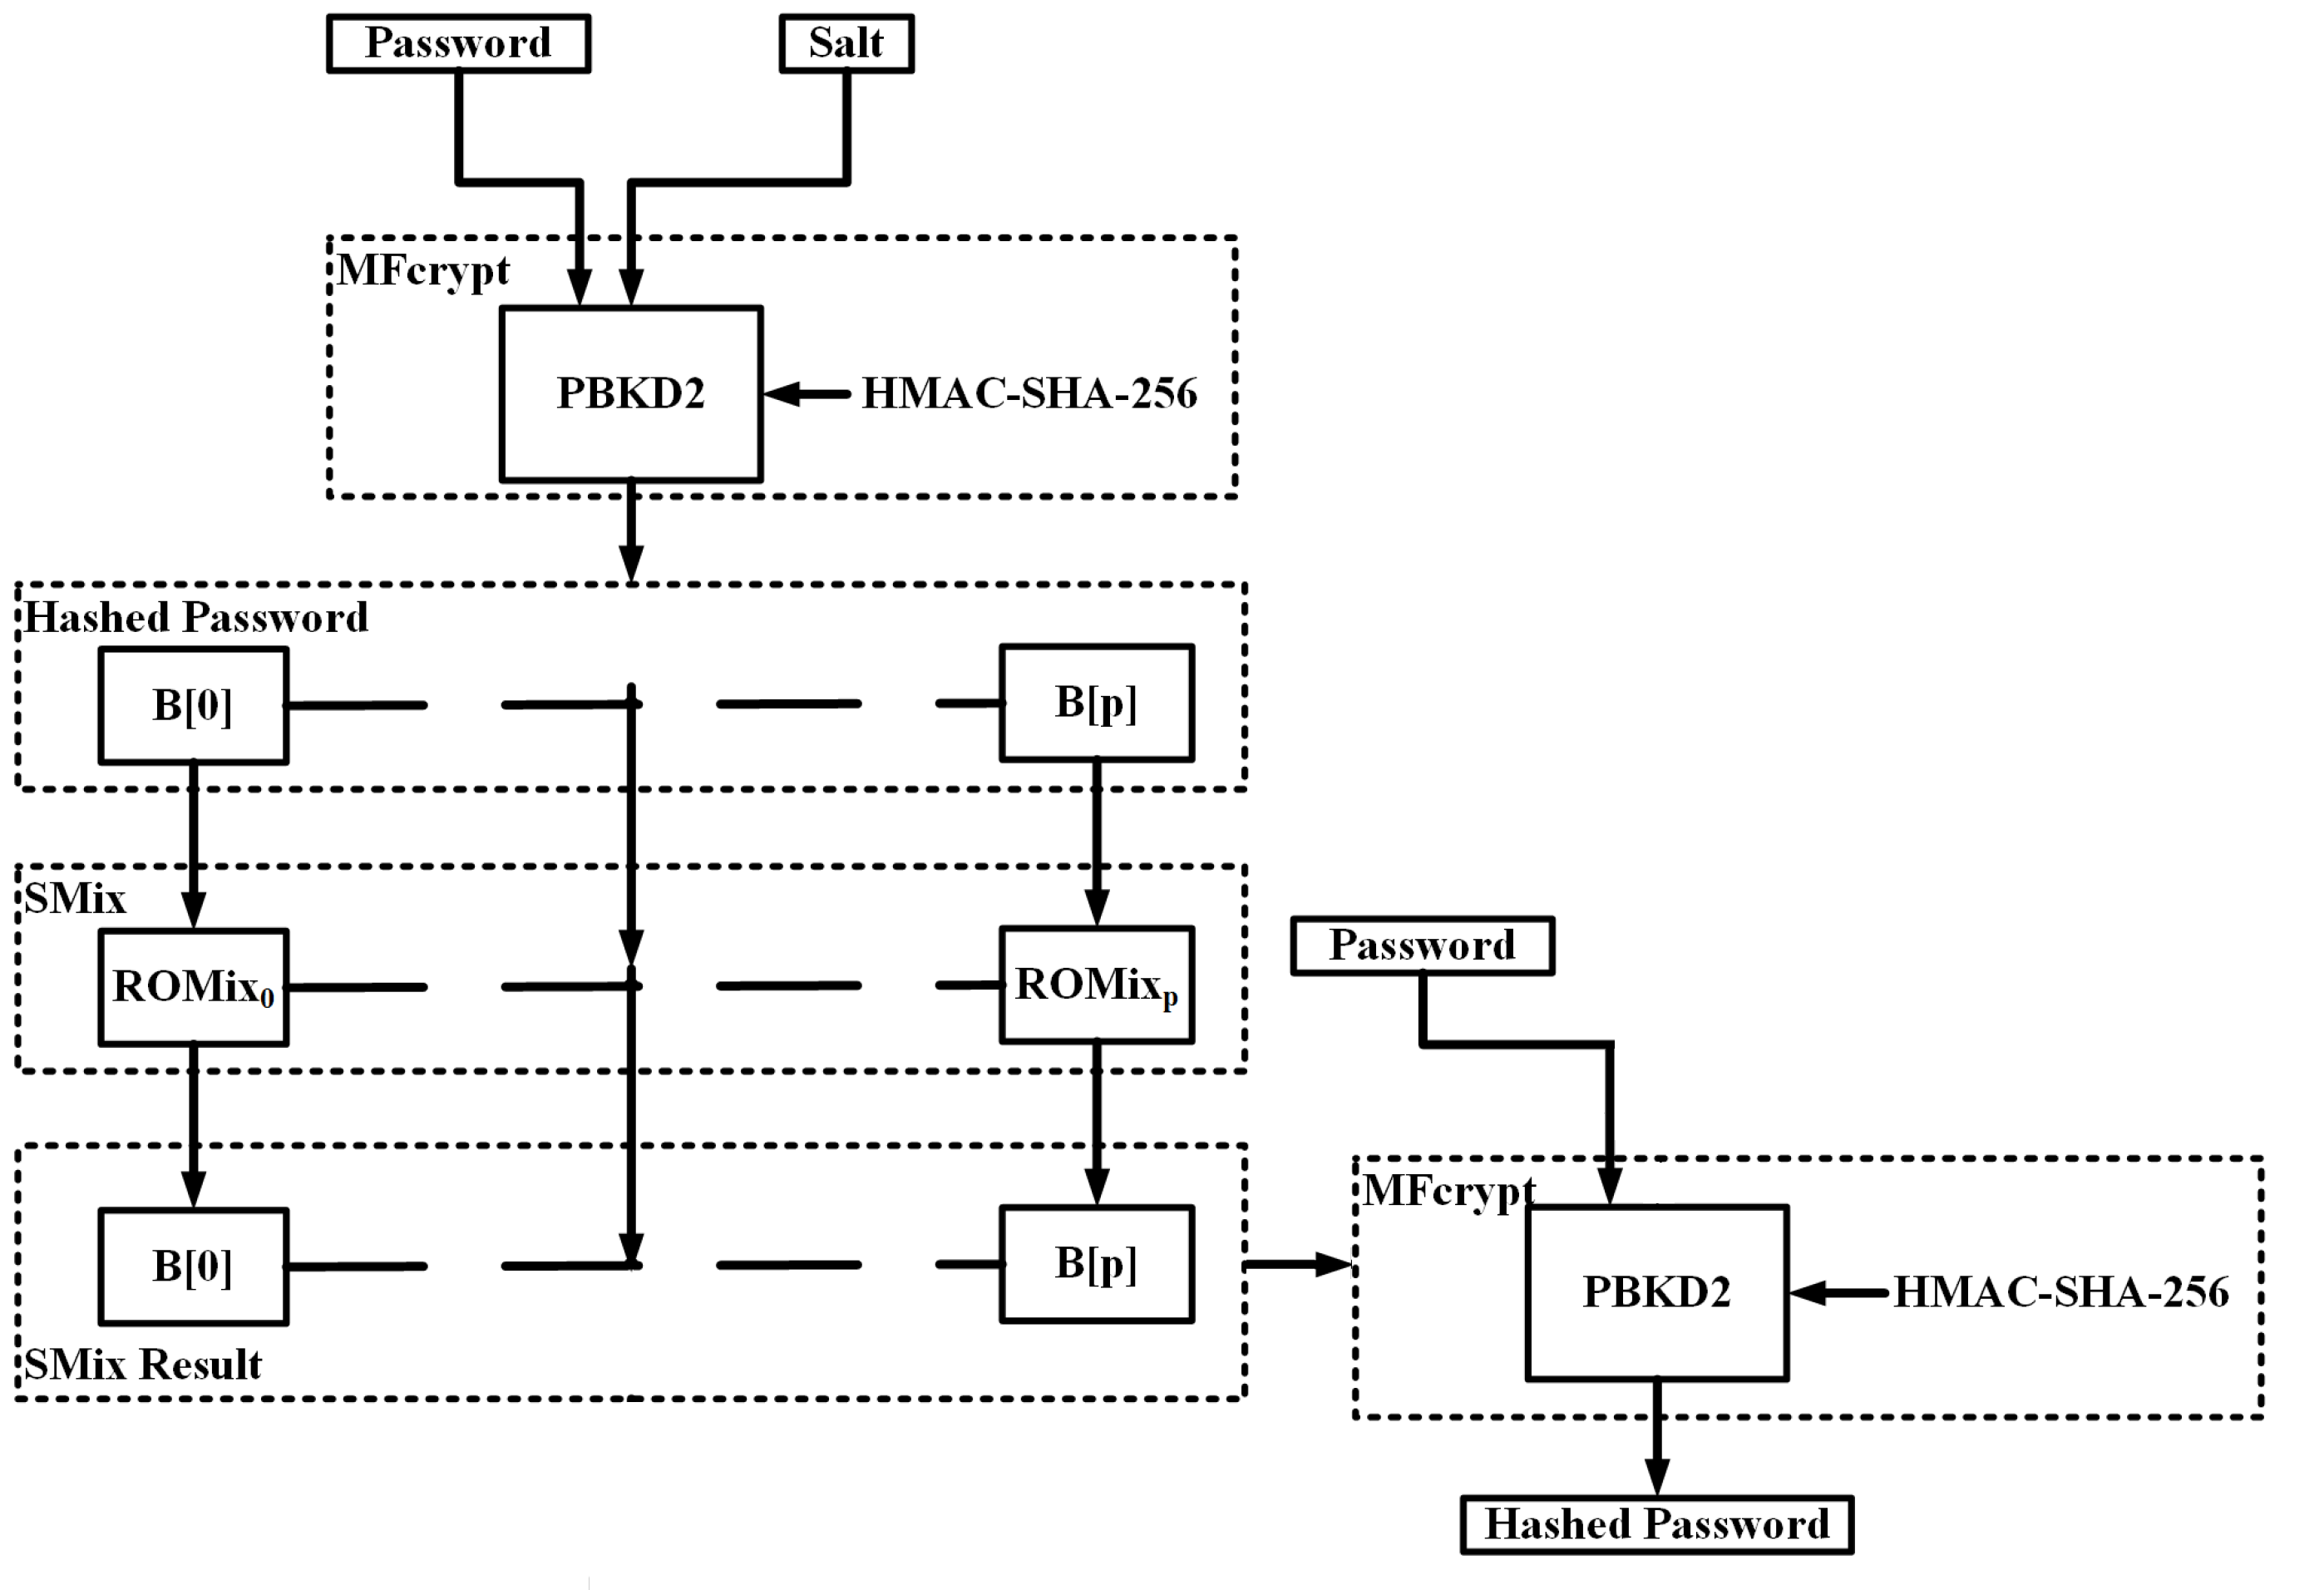
\includegraphics[scale = 0.10]{Scrypt2.png}
	\caption{Scrypt}
	\label{}
\end{figure}


\clearpage
\section{Password cracking tools}
Passwords are created by humans using recurring patterns. These patterns are taken advantage of by data-driven password cracking techniques that rely on massive password breach collections. \\\\
Nowadays, it is common practice to simulate password cracking in order to determine the strength of a password. Numerous algorithms for breaking passwords are probabilistic, which means they build a model and then give each potential password a probability. The strength of a password is proportional to the number of passwords with higher probability based to that model, assuming the attacker logically guesses passwords in descending order of likelihood. \\\\
However, probabilistic tools are rarely used by real-world attackers; instead, they mostly employ programs like Hashcat and John the Ripper (JtR).\\\\ 
They give practical explanations.
In offline attacks, the time it takes to make and check a guess includes the time to create a guess, hash it, and see if it matches the target password. Probabilistic algorithms are good at guessing passwords, but they take a lot of computer power to generate each guess. \\\\
So, for most fast hash functions, it's quicker to crack passwords using different software tools. While the likelihood of guessing a password with a probabilistic model might match the order of guessing with software tools, it's not always accurate.


The mangled-wordlist assaults of JtR and Hashcat are the most frequently used and intellectually engaging. These attacks take advantage of the fact that passwords typically vary in subtle, predictable ways; for example, a word may have a digit added to it by one person, while the same word may have a symbol added by another. In a mangled-wordlist attack, the attacker generates a rule list of mangling rules (such as appending a digit and replacing "s" with "\$") written in a transformation language given by the tool, together with a wordlist comprising popular passwords and natural language content. Every mangling rule is applied to every word in the order that the input lists specify during the whole attack.


\clearpage
\subsection{HASHCAT}
\begin{figure}[h]
	\centering
	
\includegraphics[scale = 0.20]{Hashcat.png}
\end{figure}

Hashcat is a popular password cracking tool used by security professionals and attackers to recover lost or forgotten passwords or to test the strength of passwords.
\\\\
Types of attacks:
\begin{itemize}
\item Brute-Force Attack: Hashcat can perform a brute-force attack, where it systematically tries every possible combination of characters until it finds the correct password. This method is effective but can be time-consuming, especially for longer and more complex passwords.

\item Dictionary Attack: Instead of trying every possible combination, Hashcat can use a predefined list of commonly used passwords, called a dictionary, to attempt to crack passwords. This method is faster than brute-force but relies on the likelihood that the password is contained in the dictionary.

\item Combination Attack: Hashcat can also combine both brute-force and dictionary attacks. It starts with the words in the dictionary and then appends, prepends, or replaces characters to create variations of those words, effectively expanding the search space.
    
\item Rule-Based Attack: Hashcat supports rule-based attacks where users can define custom rules to manipulate the dictionary words before attempting them as passwords. For example, rules can be created to add numbers or special characters to the end of dictionary words.
    
\item Mask Attack: This method allows users to specify a mask or template for the password, defining the possible characters and their positions. Hashcat then generates and tests passwords based on this mask.
    
\item Hybrid Attack: Hashcat can combine different attack modes to increase the chances of cracking passwords. For example, it can perform a dictionary attack with rule-based mutations.

\end{itemize}





\clearpage
\subsection{John the Ripper - JTR}
\begin{figure}[h]
	\centering
	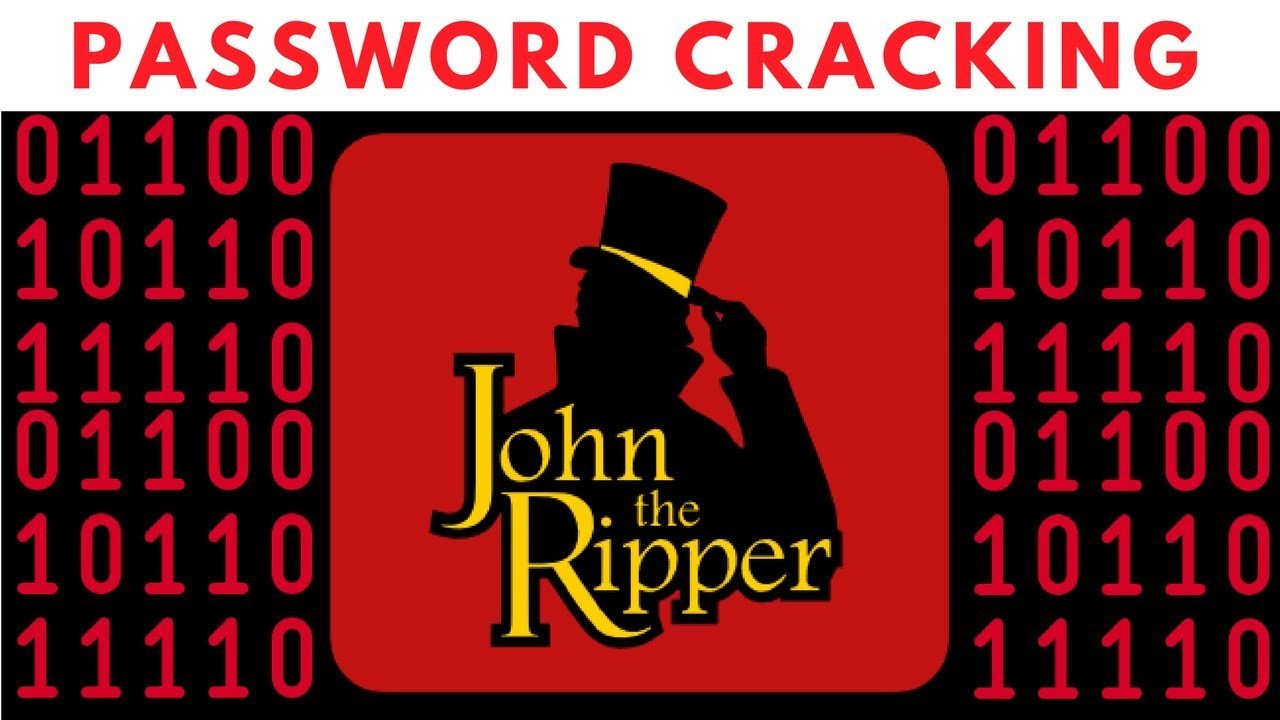
\includegraphics[scale = 0.20]{John_the_Ripper.jpeg}
\end{figure}

John the Ripper is another widely used password cracking tool utilized by security professionals and attackers alike. It operates using similar techniques as Hashcat, employing various methods to crack passwords. It is a versatile and powerful tool for cracking passwords, offering various techniques to suit different scenarios and types of passwords.
\\\\
Types of attacks:

\begin{itemize}
\item Dictionary Attack: John the Ripper can perform a dictionary attack by trying words from a predefined list of common passwords or from a custom dictionary file. It systematically checks each word in the dictionary against the hashed passwords to see if there's a match.

\item Brute-Force Attack: Like Hashcat, John the Ripper can also conduct brute-force attacks by systematically trying every possible combination of characters until it finds the correct password. This method is effective but can be time-consuming, especially for longer and more complex passwords.

\item Rule-Based Attack: John the Ripper supports rule-based attacks where users can define custom rules to manipulate the dictionary words before attempting them as passwords. For example, rules can be created to add numbers or special characters to the end of dictionary words.

\item Incremental Mode: This mode in John the Ripper generates passwords by incrementally increasing their length and complexity based on predefined rules. It starts with short passwords and gradually builds up to longer ones, trying different combinations along the way.

\item Hybrid Attack: John the Ripper can combine different attack modes, such as dictionary attacks with rule-based mutations or brute-force attacks with specific character sets.

\item Single Crack Mode: This mode allows John the Ripper to crack password hashes with just one attempt, using various techniques like dictionary, brute-force, and incremental attacks
\end{itemize}

%%%% COMMENT
\begin{comment}
JtR and Hashcat’s mangled-wordlist attacks are their most commonly used [15] and most intellectually interesting. These attacks leverage the insight that passwords tend to differ in small and predictable ways; while one person may append a digit to a word, another might append a symbol to that same word. In a mangled-wordlist attack, the attacker creates a wordlist of common passwords and natural-language content, as well as a rule list of mangling rules (e.g., replace ‘s’ with ‘$’ and append a digit) written in a transformation language specified by the tool. The full attack applies each mangling rule to each word in the order specified by the input lists.

Thus, the practical strength of a password pw is strongly affected by if and when JtR/Hashcat would guess pw, yet it is difficult to compute this information. To date, one would simply run JtR/Hashcat on a given rule list and wordlist, enumerating guesses and recording when pw is generated [8]. This has several limitations. Generating a huge number of guesses is computationally expensive, and when one stops the attack it is not known which unguessed passwords would ever be guessed. Moreover, it is unclear which rule list and wordlist an intelligent attacker should choose, and how they should be ordered. Re-running JtR/Hashcat on the myriad possible lists is intractable. Knowledge of these tools’ complex behaviors is limited to glimpses obtained via expense computations.

Our first contribution: An analytical approach to modeling transformation-based password guessing. We develop a more efficient approach for studying mangled-wordlist attacks without actually running them. We design and implement tools that analytically compute properties of JtR and Hashcat, including whether they would generate a particular password and how many guesses each rule generates. These techniques enable estimation of a password’s strength by accurately and efficiently computing how many passwords would be guessed before it in an attack using these tools in a particular configuration. We term this process a guess-number calculator. While prior work has developed guess-number calculators for Markov models [10], probabilistic context-free grammars [7], and neural networks [13], ours is the first computationally efficient approach for modeling widely used cracking software.

In particular, we develop modules for rule inversion and guess counting. Rule inversion efficiently computes a compact representation describing the preimage set of a rule for a password pw (the set of words the rule will mangle into pw). This allows one to easily see whether a rule would generate a target password with a given wordlist. Guess counting computes the number of guesses generated by a rule without running it. Both modules run much faster than naive execution.

For example, consider the task of determining whether passwords password156 and monkey! would be generated by a rule that appends two digits to every entry of a given wordlist. One could first invert that rule by attempting to remove two digits from the end of the password. If this inversion is successful (password156 becomes password1), then the task is reduced to a constant-time lookup of whether password1 is in the wordlist. If (and only if) it is, password156 would be guessed. Because monkey! does not end in two digits, we determine it cannot be guessed by that rule. We can also determine how many guesses this rule issues: 100 times the number of entries in the wordlist.

While these computations were straightforward for this simple rule, JtR and Hashcat support dozens of more complex transformations (e.g., substitutions, purging classes of characters, conditionally rejecting candidate guesses). Furthermore, a rule can compose many individual transformations. We formally analyze both tools’ full rule languages, building efficient algorithms for handling most complex rules. Our tool can invert and guess count the vast majority of transformations supported by JtR/Hashcat, as well as arbitrary compositions of transformations. However, for some rules (e.g., character purging), we must resort to brute-force execution of JtR/Hashcat.

Given a password pw, our guess calculator determines how many guesses JtR/Hashcat would issue before guessing pw. Doing so efficiently enables quick estimation of a password’s strength. After some moderate precomputation, our calculator responds in only a few seconds even for attacks making 300 trillion guesses, enabling the first real-time estimation of password strength against common mangled-wordlist attacks.
\end{comment}


\clearpage
\section{Testing - Password cracking}
Environment used: Oracle VM VirtualBox\\
OS used: \hspace{1.35cm} Kali Linux\\
Version:  \hspace{1.5cm} kali-linux-2024.1-virtualbox-amd64\\
Type of cracking: \hspace{0.05cm} Offline\\
Base Memory: \hspace{0.5cm} 4096 MB\\
Processors: \hspace{1cm} 2\\
Boot Order: \hspace{0.82cm} Hard Disk, Optical\\
Acceleration: \hspace{0.67cm} Nested Paging, PAE /NX, KVM Paravirtualization\\\\
View of Kali Linux:
\begin{figure}[h]
	\centering
	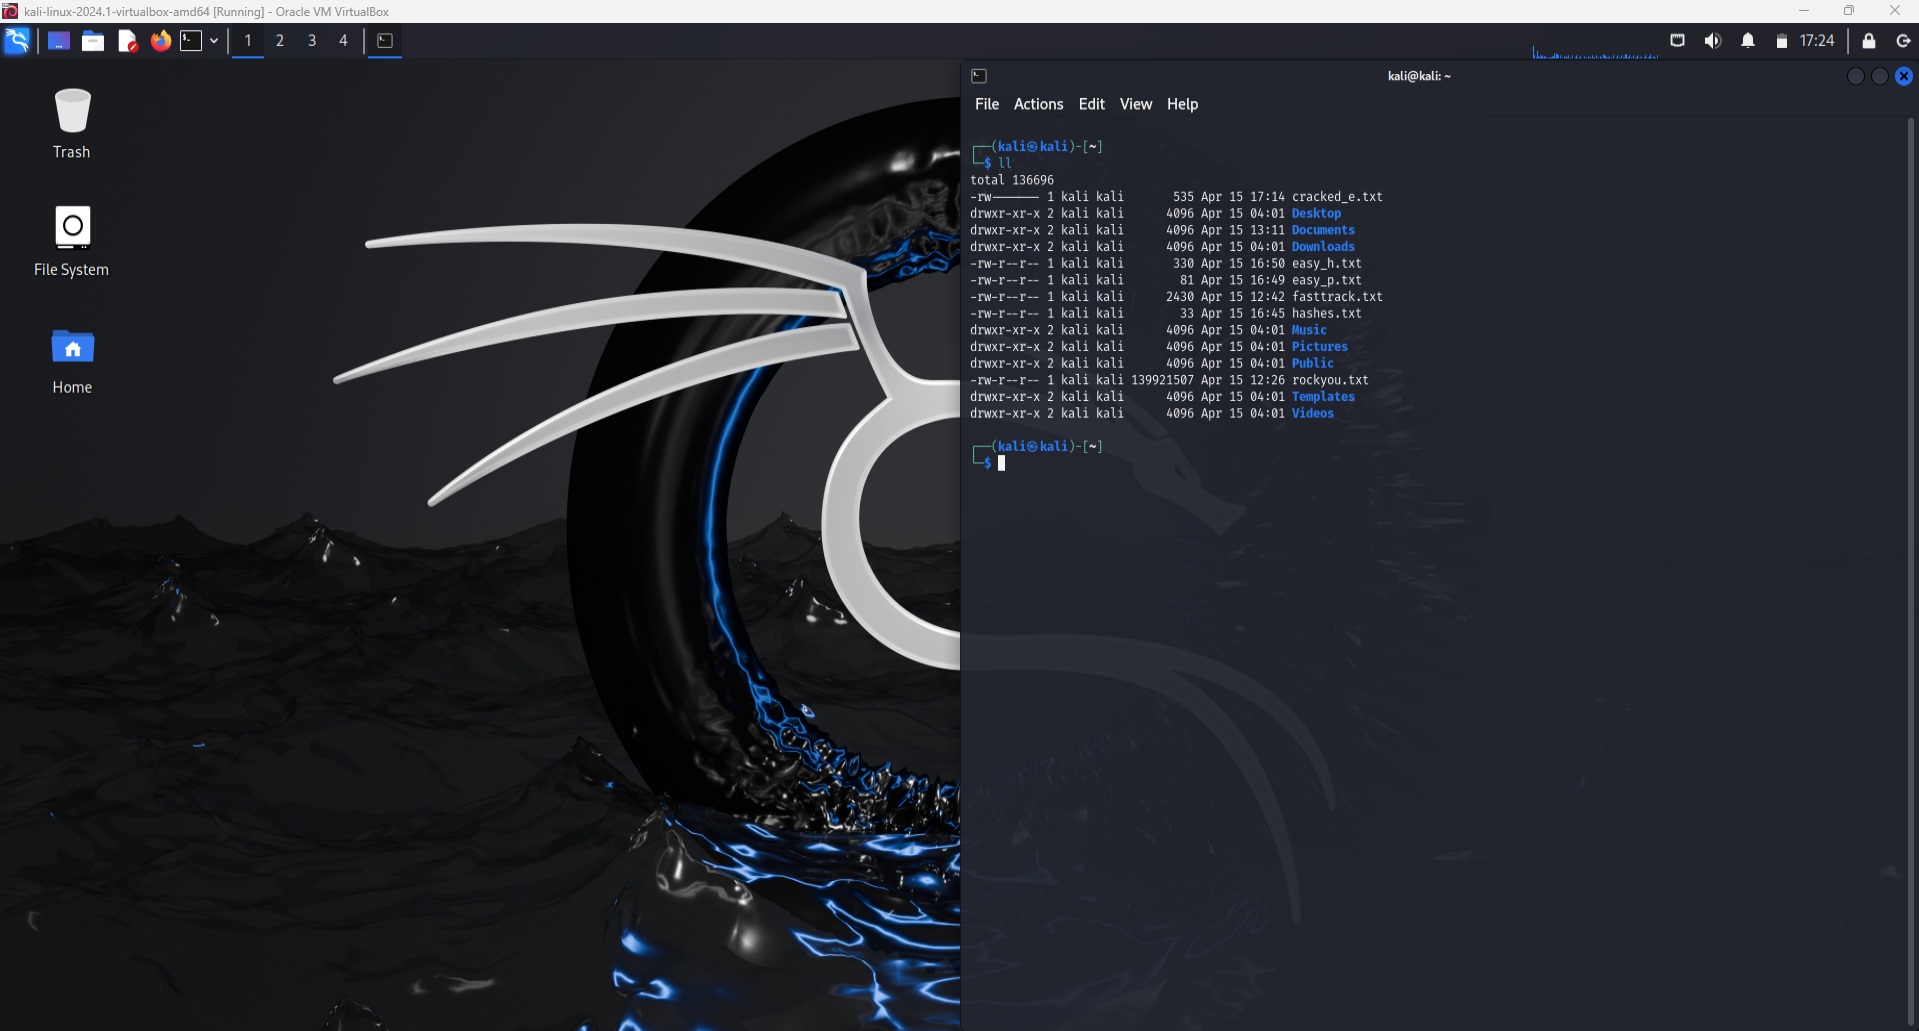
\includegraphics[scale = 0.30]{kali_terminal.png}
\end{figure}\\
- Kali Linux has more wordlists already stored and the largest of them is the rockyou.txt wordlist found in: /usr/share/wordlists/rockyou.txt.gz.\\
- After unzipping this file we have a wordlist with over 14 million (14,344,392) common passwords people use/used.\\
- The "rockyou.txt" wordlist is compiled from data breaches, primarily from a significant breach of the social networking site RockYou in 2009. During this breach, hackers gained access to RockYou's user database, which contained millions of usernames and passwords stored in plaintext. The breach exposed the weak security practices of the time, as RockYou stored passwords without proper encryption.\\
- Hashcat and John the Ripper are preinstalled with Kali, so no other installing is needed.\\



\pagebreak
\subsection{Hashcat}
- Version: hashcat (v6.2.6) \\
- hashcat - Advanced CPU-based password recovery utility
\begin{figure}[h]
	\centering
	
\includegraphics[scale = 0.10]{Hashcat.png}
\end{figure}\\
- How to use Hashcat:\\\\
hashcat [options] hashfile [mask|wordfiles|directories]\\
-a, --attack-mode=NUM\\
-m, --hash-type=NUM\\
--potfile-disable, hashcat puts already cracked passwords in a pot file (basically saying: i dont need to crack these, i already cracked them, i am going to save time)\\\\
- Attack modes:
\begin{itemize}
	\item 0 = Straight
	\item 1 = Combination
	\item 3 = Brute-force
	\item 6 = Hybrid Wordlist + Mask
	\item 7 = Hybrid Mask + Wordlist
\end{itemize}
- Hash types: total 93 hash types to choose from
\begin{itemize}
	\item for example: MD5, HMAC-MD5, SHA1, NTLM, SHA256, Plaintext ...
\end{itemize}
- Example usage - cracking password hash, hash type - SHA256, mode - straight:
\begin{figure}[h]
	\centering
	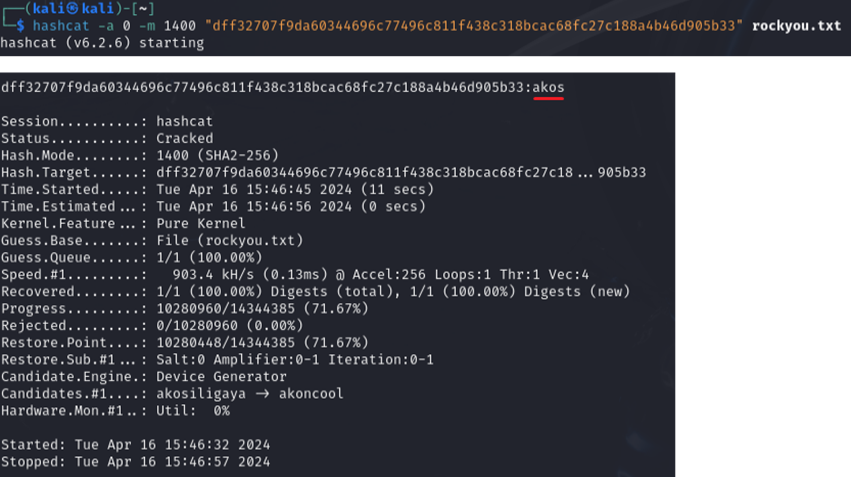
\includegraphics[scale = 0.70]{test_hashcat_akos.png}
\end{figure}\\\\
%Tested cracking with different hashing algorithms - md5, sha-256, sha-1, bcrypt\\
%Tested cracking with different lengths of passwords - 5, 10, 15\\
%Tested cracking with different types of attacks - straight, wordlist, brute force\\

- Different lengths for the passwords and different types of hashes used:\\
\begin{figure}[ht]
	\centering
	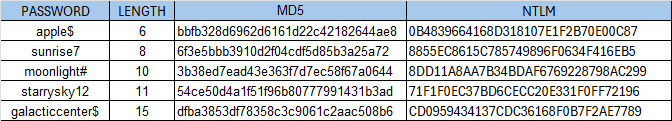
\includegraphics[scale = 0.60]{diff_md5_ntlm.png}
\end{figure}
\begin{figure}[ht]
	\centering
	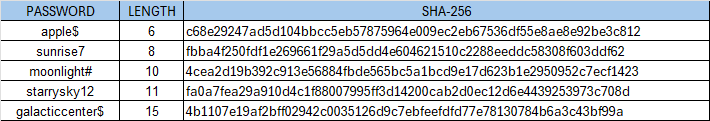
\includegraphics[scale = 0.60]{diff_sha.png}
\end{figure}

- Testing the passwords with hashcat:\\\\
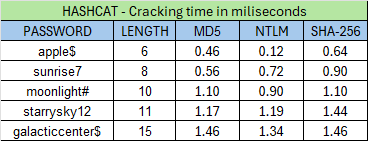
\includegraphics[scale = 0.70]{diff_hashcat.png}\\

- Testing the passwords with john the ripper:\\\\
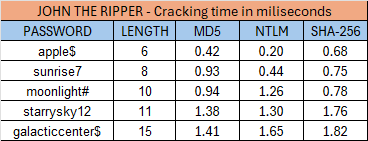
\includegraphics[scale = 0.70]{diff_jtr.png}



\pagebreak
\subsection{John the Ripper}
- Version: John the Ripper 1.9.0-jumbo-1+bleeding-aec1328d6c\\
- john - a tool to find weak passwords of your users
\begin{figure}[h]
	\centering
	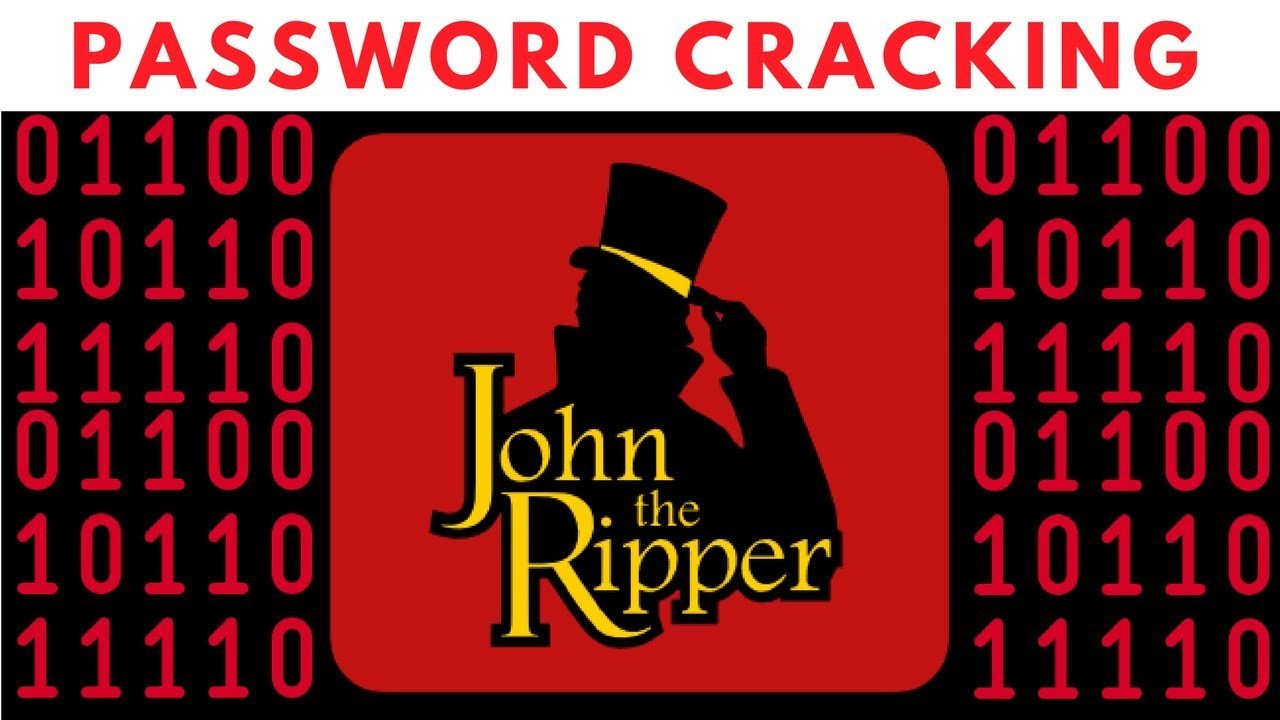
\includegraphics[scale = 0.10]{John_the_Ripper.jpeg}
\end{figure}\\
- How to use John the Ripper:\\\\
john [options] password-files\\
--format:NAME, Allows to override the ciphertext format detection. (Currently, valid format names are  DES,  BSDI, MD5,  BF,  AFS,  LM)\\
--format=raw-[hash type]\\
--[MODE]\\\\
- Attack modes:
\begin{itemize}
	\item --single
	\item --wordlist:FILE
	\item --incremental[:MODE]
\end{itemize}
- Example usage - cracking a password hash for a .zip file:
\begin{figure}[h]
	\centering
	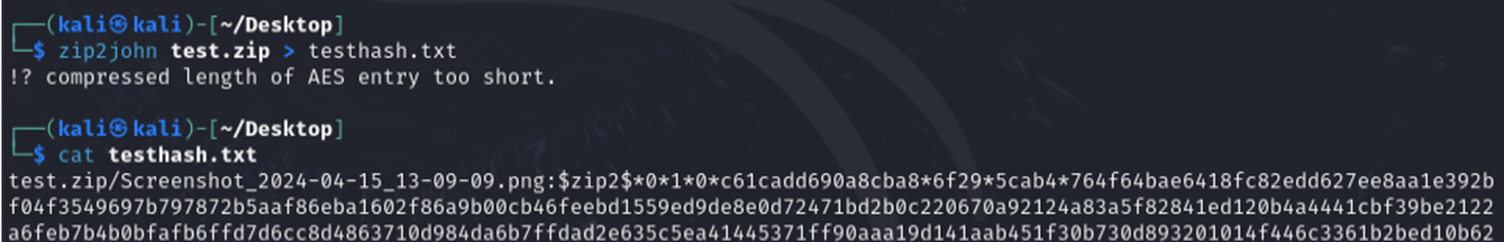
\includegraphics[scale = 0.50]{jtr_zip.png}
	\centering
	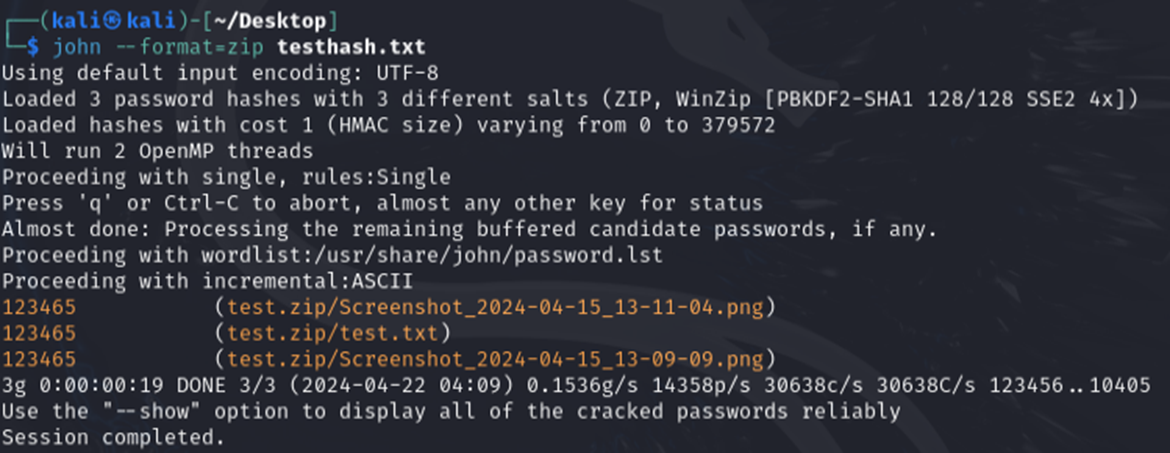
\includegraphics[scale = 0.50]{jtr_zip_2.png}
\end{figure}\\


\clearpage
\subsection{Comparing Hashcat vs John the Ripper}
- Testing the speed of Hashcat and John the Ripper with different hash types and different strengths for passwords:
\begin{figure}[h]
	\centering
	%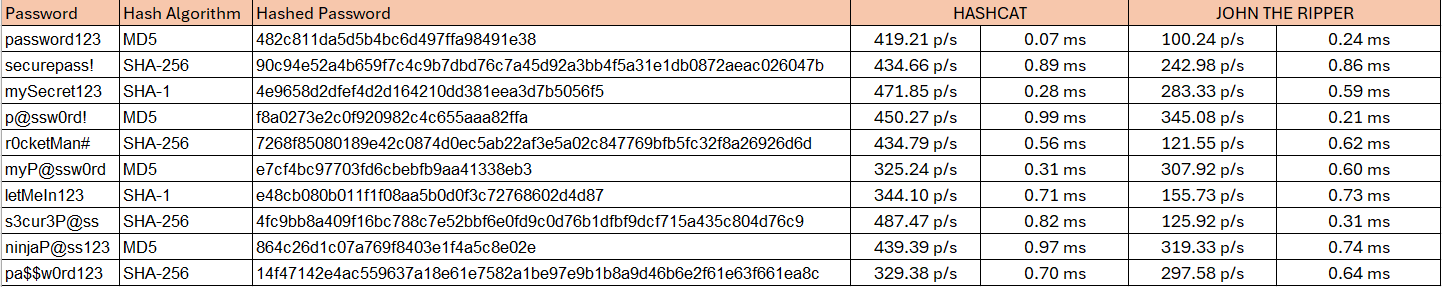
\includegraphics[scale = 0.42]{compare_table_hashcat_jtr.png}
    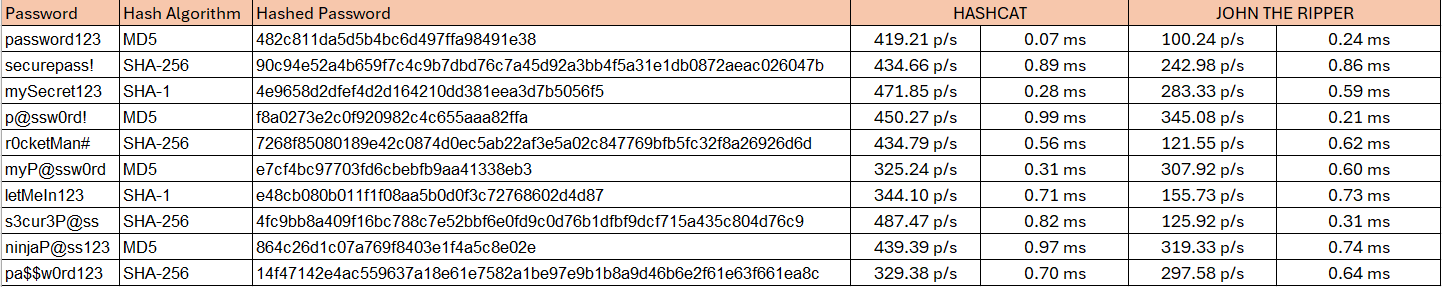
\includegraphics[width=1.3\textwidth, height=1.1\textheight, keepaspectratio]{compare_table_hashcat_jtr.png}
\end{figure}
\begin{itemize}
\item Speed
\begin{itemize}
\item Hashcat is generally faster than John the Ripper because it is optimized for working with a wide range of hardware accelerators like GPUs (graphics processing unit) and FPGAs (Field programmable gate array). This allows Hashcat to perform high-speed brute-force attacks, combinatorial attacks, and more, using the massive parallel processing power of modern GPUs.
\item John the Ripper has a mode called Jumbo that supports GPU acceleration, but its primary strength lies in CPU-based attacks. John's performance can be very good on CPUs, but typically, Hashcat outperforms John when it comes to GPU acceleration.
\end{itemize}

\item Ease of Use
\begin{itemize}
\item Hashcat has a steep learning curve due to its extensive range of options and configurations, which can be overwhelming for beginners. However, it has a consistent syntax and well-documented options, which, once mastered, can be highly effective and flexible.
\item John the Ripper is often considered easier for beginners, especially in its default mode. It automatically selects the best strategies and algorithms based on the hashes it detects, which simplifies the process for new users. However, making full use of its capabilities (especially in Jumbo mode) still requires learning a variety of options and configurations.
\end{itemize}

\item When to Use Which
\begin{itemize}
\item Use Hashcat when:\\
You have access to powerful GPUs and need to perform high-speed, high-volume cracking.\\
You are dealing with a very large set of hashes or need to use advanced attack modes that leverage GPU power.\\
You need to crack hashes that are better supported by Hashcat's more modern algorithms and optimizations.\\
\item Use John the Ripper when:\\
You are working on a system with limited or no GPU resources.\\
You need a tool that's good at automatically handling different hash types with minimal configuration.\\
You are engaging in pentesting scenarios where you might benefit from the flexibility and scriptability of John the Ripper, especially with custom rules and modes designed to crack complex password patterns.\\
\end{itemize}
\end{itemize}


\section{Passwords Strength}
When passwords are compromised, it can lead to serious consequences such as personal information exposure, financial losses, and theft of sensitive data. As Internet technology advances, users are required to manage an increasing number of passwords. However, creating strong passwords that are also easy to remember is challenging. Consequently, users may resort to using personal information like names, birthdates, or phone numbers, making them vulnerable to targeted attacks and password reuse. Balancing security and usability has become a challenge for users.\\
Strength of a password is determined by a number of variables, such as length, complexity, randomness, and character set. 
The ways in which these elements affect password strength are broken down here:
\begin{itemize}
\item Length: Because they give hackers more room to search, longer passwords are typically more secure than shorter ones. 
The number of combinations that are feasible increases exponentially with each extra character. 
\begin{itemize}
        \item With simply lowercase letters, there are 268268 potential permutations for an 8-character password.
        \item There are 26122612 potential permutations for a 12-character password using the same character set, which is a far bigger number.
\end{itemize}


\item Character Set: Adding a range of characters to your password, such as digits, special characters, lowercase and uppercase letters, and numbers, makes it more difficult to crack and less vulnerable to brute-force attacks.
\begin{itemize}  
	\item Since "password" is a single lowercase letter, it is a weak password.
	\item Because it combines capital and lowercase letters, numerals, and special characters, a password like "P@ssw0rd!" is more robust than others.
\end{itemize}

\item Randomness: Passwords that are generated at random tend to be more secure than those that are based on popular terms or patterns. Dictionary or pattern-based attacks are less likely to guess or break random passwords.

\item Predictability Avoiding: Keeping your password strong means staying away from patterns or sequences that are simple to figure out (like "123456" or "qwerty"). To further improve security, keep personal information like names, birthdays, and frequent words to a minimum.
\end{itemize}
Here are some examples demonstrating the impact of length and complexity on password strength:
\begin{itemize}
    \item Weak Password: "password"
	\begin{itemize}
       \item Length: 8 characters
       \item Character Set: Lowercase letters only
       \item Strength: Very weak, easily guessable or crackable
	\end{itemize}
    \item Moderate Password: "P@ssw0rd"
	\begin{itemize}
       \item Length: 8 characters
       \item Character Set: Uppercase letters, lowercase letters, digits, special characters
       \item Strength: Moderate, resistant to basic attacks but still vulnerable to advanced techniques
	\end{itemize}
    \item Strong Password: "Tr0ub4dor\&3"
	\begin{itemize}
       \item Length: 12 characters
       \item Character Set: Uppercase letters, lowercase letters, digits, special characters
       \item Strength: Strong, significantly increases the search space for attackers and provides good resistance to various attack methods
	\end{itemize}
    \item Very Strong Password: "x\#uT7f\^rB2@j\$LmP"
	\begin{itemize}
       \item Length: 16 characters
       \item Character Set: Uppercase letters, lowercase letters, digits, special characters
       \item Strength: Very strong, extremely difficult to crack due to length and complexity
	\end{itemize}
\end{itemize}

\pagebreak
\section{Password Managers}
Password managers are software tools designed to securely store and manage passwords for various online accounts and services.\\They work by encrypting and storing your passwords in a centralized vault, which is typically protected by a master password or passphrase. \\When you need to log in to a website or app, the password manager can automatically fill in the credentials for you, saving you the trouble of remembering or typing them manually.

\begin{itemize}
\item Password Storage: The password manager safely saves your login information in an encrypted database or vault whenever you establish an account or change a password.
\item Password Master: You just need to remember one master password or passphrase in order to access the password manager and recover your stored passwords. The password vault must be unlocked using this master password.
\item Encryption: To protect your passwords and other private data, password managers employ robust encryption methods. This guarantees that the stored data cannot be accessed without the master password, even in the event of unwanted access.
\item Auto-fill and Auto-generate: When you visit a website or open an app, password managers can automatically fill in login fields for you. This is a function that many of them come with. To provide increased protection, they can also create powerful, randomized passwords for brand-new accounts.
\item Cross-Platform Syncing: You can access your passwords from your computer, smartphone, or tablet with the help of many password managers that support synchronization across various devices.
\item Browser Extensions and Apps: To facilitate cross-platform and cross-device use, password managers usually provide browser extensions or stand-alone apps that interface with your operating system or web browser.
\end{itemize}



\clearpage
\bibliography{literature}
\bibliographystyle{plainurl}
\nocite{*}

\end{document}

